\documentclass[10pt,journal,compsoc]{IEEEtran}


\hyphenation{op-tical net-works semi-conduc-tor}

\usepackage[sorting=ydnt,backend=bibtex]{biblatex}
\addbibresource{bibliography.bib}
\usepackage{listings}
\usepackage{graphicx}
\usepackage{hyperref}

\begin{document}

\title{Overview - ``A Wait-free Queue as Fast as Fetch-and-Add''}

\author{Loris~Lucido\\\small{\textit{Author:} Chaoran~Yang,
        John Mellor-Crummey}}% <-this % stops a space}

\IEEEtitleabstractindextext{%
\begin{IEEEkeywords}
non-blocking queue, wait-free, fast-path-slow-path
\end{IEEEkeywords}}

\maketitle

\IEEEdisplaynontitleabstractindextext
\IEEEpeerreviewmaketitle

\newcommand{\para}[1]{\textbf{\textit{#1}}\hspace{2 mm}}

\section{Introduction}\label{sec:introduction}
Fast concurrent data structures are necessary to exploit the power of multi-core
processors and multiprocessors machine. To deliver high scalable performance,
applications may need shared objects (data structures) whose operations are
scalable. Each operations of an object (adding, removing, modifying an element)
much perform \textit{reasonably} well even when the number of threads sharing an
object is high.

One way to construct concurrent data structures is by using an object with
blocking operations. An example of such object would be a concurrent queue whose
operations have been protected with mutual exclusion (locks). This approach is
not scalable and it will lead to poor performance under high contention,
especially if the application uses more software threads than hardware threads.
Unexpected delay from one thread prevents the others to use the object. The
source of the delay is multiple : operating system preemption, cache miss, page
fault, etc. Therefore designing non-blocking objects is the topic of lots of
past and ongoing researches. \\

\para{Wait-free object} We define here levels of process guarantees

on each operation of a non-blocking object \cite{Yang:2016:WQF:3016078.2851168}.
Those are meant to predict how an object will behave under high contention. The
strongest guaranty is wait-free, which means an operation will complete in a
finite number of steps regardless of how many threads is accessing this object
and at what speed. Lock-free operations complete in a finite number of steps
only for \textit{some} threads while it may not be the case for the others.
Obstruction-free is the weakest guaranty. Only one thread is guaranteed to
complete an operation in a finite number of steps.

While an object can be wait-free, this doesn't mean it will enable the
application to achieve high scalability. Actually, (*reference*) most past
wait-free queue implementations perform worse than others lock-free or blocking
queue. To achieve a wait-free guarantee, most wait-free implementations have to
either sacrifice parallelism or linearizability. \\

\para{Linearizability} Having multiple threads concurrently modifying a shared
object must not leave this object (a queue for example) in an
\textit{inconsistent} state. To ensure the designed object is correct, we need a
correctness condition for shared objects. The authors choose linearizability for
their design of concurrent queue. Each operation must appear to \textit{take
effect} instantaneously from the point of view of other threads. The order of
non-concurrent operations must also be preserved, regardless of when the
operation started and ended \cite{Herlihy:1990:LCC:78969.78972}.

An atomic operation or an operation protected by mutual exclusion is by
definition linearizable. When the operation is not atomic, one must consider the
point in time when changes made to the shared object become visible to the other
threads.

paragraphe sur coherence sequentiel ? \\

\para{Memory reclamation} Memory management is an important part of designing a
concurrent non-blocking algorithm. Garbage collection is not available in all
languages and, even it exists, one may need to do his own memory management to
be more efficient, especially if the garbage collection process is not lock-free
or wait-free.

The use of \texttt{malloc}, for example, may also violate the wait-free property
of the queue because \texttt{malloc} uses mutual exclusion to manage memory. One
solution is to have each thread manages a pool of pre-allocated cells
\cite{Herlihy08}. Enqueue operation take one cell from the pool, dequeue
operation put the cell back into the pool. While this solution avoids lock
contention, it is proned to the ABA problem which may corrupt memory.

The ABA problem occurs if one thread reads a shared address $A$, attempts to
replace the value of this cell with a compare-and-swap ($CAS$) and succeeds when
it should not. For example, if between the read and the comparison, another
thread replaced $A$ to $B$, and then replaced $B$ to $A$ again, the
compare-and-swap should fails.

One can also use other memory management implementations like \texttt{jemalloc},
\texttt{TCMalloc}, or \texttt{Lockless}. \\

\para{Consensus number} The use of atomic primitives such as compare-and-swap is
critical in designing Lock-free algorithm. To understand why, we must consider
the consensus problem. A consensus is reached between $n$ threads if those $n$
threads can \textit{decide} on a value : each thread proposes one value to the
others and then chooses one value. The consensus is reached if all threads
decides the same value (consistency requirement) and if the common decision is
one of the initially proposed value (validity requirement).

Compare-and-swap primitive has an infinite consensus number
\cite{Herlihy:1991:WS:114005.102808} : it can solve the consensus problem for an
infinite number of threads. Compare-and-swap holds another important property
which is universality. An object is universal for $n$ threads if and only if it
has a consensus number greater or equal to $n$. It is possible to implement any
concurrent object in a wait-free manner if and only if the operation system
provides an universal object. Thus, compare-and-swap can be used to implement
any arbitrary concurrent wait-free object for any number of threads. This
statement holds for other infinite consensus number primitive like
load-linked/store-conditional. \\

\para{Contribution} Unfortunately, the use of compare-and-swap on a variable
shared by several threads can drastically reduce performance even under low
contention (compare-and-swap retry problem
\cite{Morrison:2013:FCQ:2517327.2442527}). In this paper, Yang C. and
Mellor-Crummey J. expose a new queue that is wait-free, linearizable, and
delivers high performance.

They avoid common issues with past designs such as the compare-and-swap problem
by also relying on a fetch-and-add primitive ($FAA$). Fetch-and-add has
consensus number two but is less expensive than compare-and-swap and cannot
fail. They designed their wait-free queue using a methodology called
fast-path-slow-path \cite{Kogan:2012:MCF:2370036.2145835}. It can transform
non-blocking lock-free queue implemented with compare-and-swap primitive to a
wait-free one. They adapted it for queues also using fetch-and-add. They also
provide their own memory reclamation scheme which adds little overhead unlike
previous work.


\section{Context and Related Work}\label{sec:context}
\para{MS-Queue} The MS-Queue from Michael M. M. and Scott M. L. is a classical
simple lock-free queue implemented with only compare-and-swap as primitive
\cite{Michael96simple}. Their queue is designed as a singly-linked list, with
two references to the head and the tail of the queue. Their use compare-and-swap
to add (or remove) an element to the queue and to move the head and tail
reference. As a consequence, it is subject to the compare-and-swap retry
problem. Even with a low number of threads, performance are drastically reduced
under contention because of high probability of compare-and-swap failures.

The MS-Queue avoids the ABA problem by using double width compare-and-swap. Each
compare-and-swap to an address also increments a counter associated with that
address so that the comparison is done with one address and an integer
\cite{Herlihy08} \cite{Michael96simple}. \\

\para{Practical wait-free queue} One of the first implementation of a wait-free
queue supporting multiples enqueuers and dequeuers was designed by Kogan A. and
Petrank E. \cite{Kogan:2011:WQM:2038037.1941585}. This queue is based on the
MS-Queue. Each operation is divided into three atomic steps, threads can help
each others to complete a step without letting the possibility for steps
interleaving among the same type of operation (enqueue or dequeue). Because of
the overhead of this helping mechanism, it doesn't perform as well as the
MS-Queue. \\

\para{Combining-based queue} The P-Sim queue (wait-free) and CC-Queue (blocking)
from Fatourou P. and Kallimanis N. D. uses \textit{operation combining} to try
to achieve better scalability than compare-and-swap-based queue by reducing
synchronisation cost \cite{Fatourou:2011:HWU:1989493.1989549}
\cite{Fatourou:2012:RCS:2370036.2145849}. To do so, threads don't directly
modify the queue but publish a request. A single thread browses a list of
pending operations and applies them serially on the queue. While the CC-Queue
performs better than the P-Sim queue, it is still a blocking object and, also
because of the lack of parallelism, the CC-queue doesn't scale well. \\

\para{$FAA$-based LCRQ} The LCRQ is a lock-free queue designed by Morrison A.
and Afek Y. \cite{Morrison:2013:FCQ:2517327.2442527}. It is implemented as a
circular ring queue. Threads use fetch-and-add to get a cell index on the queue,
enqueue and dequeue are then done with double width compare-and-swap, which is
not universally available. However, by also relying on fetch-and-add, this queue
avoids the compare-and-swap retry problem. \\

\para{Fast-path-slow-path} The fast-path-slow-path methodology objective is to
construct a wait-free algorithm from a lock-free one
\cite{Kogan:2012:MCF:2370036.2145835}. This methodology relies on a
compared-and-swap-based lock-free algorithm \textit{most} of the time
(fast-path), and switch to a wait-free algorithm when too many compared-and-swap
failures are encountered by using an helping mechanism (slow-path). It aims to
achieve lock-free performance with a wait-free guaranty. They use the lock-free
MS-queue as the fast path.


\section{Contribution of the Article}\label{sec:contribution}
A basic obstruction-free queue is given in Listing \ref{lst:queue}. From this
queue, the authors construct a wait-free queue by using the fast-path-slow-path
methodology. This queue is similar to the base used in the LCRQ algorithm.

$FAA(x, v)$ atomically reads the value stored in the $x$ variable, and
increments it by $v$. $CAS(x, t, v)$ atomically reads the value stored in $x$,
compares it to $t$ and, if $x$ is equal to $t$ (success), replaces the value of
$x$ by $v$. $CAS$ returns whether it has successfully replaced the value or not.

\begin{lstlisting}[mathescape,
                   frame=single,
                   caption={An obstruction-free queue using an infinite array.},
                   label={lst:queue},
                   language=C]
Q: queue
T: pointer to tail
H: pointer to head
enqueue(x: var) {
  do t := FAA(&T, 1);
  while (!CAS(&Q[t], $\bot$, x));
}
dequeue(x: var) {
  do h := FAA(&H, 1);
  while (!CAS(&Q[h], $\bot$, $\top$) and T > h);
  return (Q[h] == T ? EMPTY : Q[h]);
}
\end{lstlisting}

\para{Basic queue} This queue uses a shared (emulated) infinite array to
store elements. We will see later how this is done and how memory can be
reclaimed. Two special values are reserved : $\bot$ (bottom) and $\top$ (top).
$\bot$ stands for empty cells as the queue is initially filled with $\bot$.
$\top$ stands for unusable cells. When one thread dequeues an element, it marks
the cells with $\top$ to prevent other threads to enqueue an element in it.

To enqueue an element, one thread tries to find an available cell on the array,
a cell marked with $\bot$. One cannot enqueue an element in a $\top$ marked cell
because it could violate the FIFO property of the queue. To get a unique index
on the array, one thread uses fetch-and-add to increment the shared tail
reference. Considering the reference is shared by all threads, using
compare-and-swap instead of fetch-and-add would result in lots of failures.
After one thread is given a unique index, it needs to certify that the cell is
empty. He then uses compared-and-swap to enqueue an element into the array. In
the event of compare-and-swap failure, the thread redoes the whole process until
the element is enqueued.

The dequeue operation works in a similar manner, one thread tries to find either a
cell filled with an element or marked with $\top$ by using fetch-and-add on a
shared head reference. If a thread stops on a $\top$ marked cell, the dequeue
returns \texttt{EMPTY}.

This queue is designed to be fast. Dequeue may always fail if queued values are
dequeued by another thread. Enqueue may always fail if another thread marks each
empty cell unusable. As a result, it is neither wait-free or lock-free because
it is prone to livelocking. As only one thread is guaranteed to progress, this
queue is only obstruction-free. \\

\begin{figure}
    \caption{The fast-path-slow-path methodology \cite{Kogan:2012:MCF:2370036.2145835}.}
    \label{fig:fpsp}
    \center
    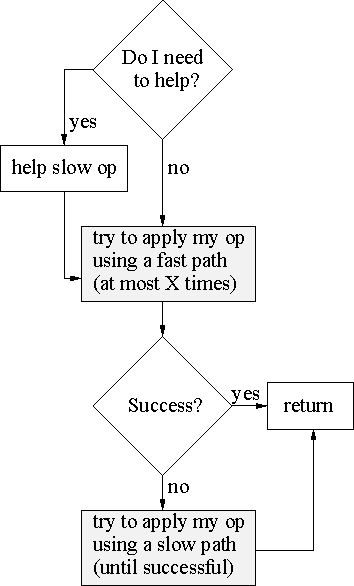
\includegraphics[width=0.6\linewidth]{img/fpsp.pdf}
\end{figure}

\para{Fast-path-slow-path} To construct a wait-free realization of the previous
queue, the authors use the fast-path-slow-path methodology. As shown in figure
\ref{fig:fpsp}, one thread tries to enqueue or dequeue an element using a
fast-path, which is similar to the previous queue. A maximum number of failures
is set. If a thread failed too many times to apply its operation, it falls back
on a slow-path.

For example, if a thread fails to enqueue an element, it publishes an enqueue
request. When other threads want to dequeue an element, they look at all pending
enqueue requests, and eventually help one request to complete. The enqueuer
thread then keeps trying to enqueue the element until it or another succeeds.

Threads are linked in a ring, they keep a reference to a \textit{peer} to which
they help the operation to complete. Each time a thread successfully helps
another thread, it updates his \textit{peer} to the next thread in the ring so
that each
thread happens to help every one at some point. \\

\para{Memory reclamation} The authors designed their queue with an infinite
array. To do so, the queue is split into segments as a linked list. Each segment
contains a fixed number of cells. The list of segments is expanded as necessary.
Because the tail and head pointers are never decremented, segments no longer in
use need to be freed.

After one thread dequeues an element, the thread tries to reclaim memory from
unused segments. They use compare-and-swap to achieve mutual exclusion so that
if several threads try to reclaim memory, only one should succeed. Unused
segments are segments filled with $\top$ marked cells. Each thread keeps a
reference to its currently used segment. The \textit{cleaner} thread ensures
that no thread keeps a reference to a segment about to be freed and changes it
if needed. \\

\para{Wait-free guaranty} The number of tries on the lock-free fast-past is
bounded. After sufficient failures, the algorithm falls back on the slow-path.
Each thread helps every other thread at some point. If the operation of one
thread continuously fails to complete, it will definitely complete when all
other threads become his helper.


\section{Discussion}\label{sec:discussion}
Fetch and Add can fails (at hardware level)

DEBRA thread failure for memory reclamation


\section{Conclusion}\label{sec:conclusion}
their design can serve as an example of how to create other wait-free object


\printbibliography

\end{document}
